\section{Turing machines}

Informally, an \emph{algorithm} is a collection of simple instructions for carrying out some task. Algorithms ahve been intuitively understood for thousands of years (for example, Euclid's algorithm), but it is not until the last couple centuries that we have formalised the notion. 

\textcite{turingComputableNumbersApplication1936} defined the now ubiquitous sequential model of computation in 1936, with the primary motivation behind his construction to capture the notion of \emph{computability}; that is, given a problem, does there exist an \emph{algorithm} that can solve it?

First, a model of computation is an abstract framework that we use to study computation; that is, how an output of a mathematical function may be computed given an input. \emph{Turing machines} are a model of computation, it is a primitive machine that is (by the Church-Turing thesis) able to run any algorithm. Turing machines are not of practical interest; they are designed to be simple to allow us to study properties of computation.

A Turing machine has infinite tape (memory). There is a finite-state \emph{program} that controls a tape head. The head can read, write, and move around in both directions on the tape. Figure \ref{fig:turing-machine} gives a visual representation of a Turing machine.


\begin{figure}
  \centering
  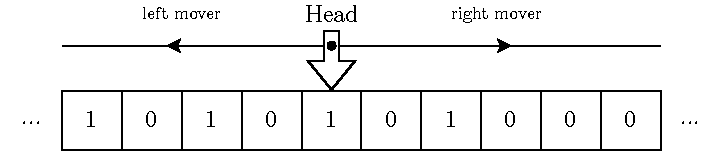
\includegraphics[width=0.8\textwidth]{content/3-complexity/images/turing-machine}
  \caption{Schematic of a Turing machine.}
  % \label{fig:turing-machine}
\end{figure}

\begin{definition}[Turing machine]
  A Turing machine is a 7-tuple \[(Q, \Sigma, \Pi, \delta, q_0, q_a, q_r)\] where
  \begin{itemize}
    \item $Q$ is a finite non-empty set of states;
    \item $\Sigma$ is the input alphabet not containing the special blank symbol $\sqcup$;
    \item $\Pi$ is the tape alphabet satisfying $\Sigma \subset \Pi$ and $\sqcup \in \Pi$;
    \item $\delta: Q \times \Pi \to Q \times \Pi \times \{L, R\}$ is the transition function;
    \item $q_0 \in Q$ is the initial state;
    \item $q_a \in Q$ is the accept state; and
    \item $q_r \in Q$ is the reject state ($q_a \neq q_r$).
  \end{itemize}
\end{definition}


We now describe computation on a Turing machine. The tape content is unbounded but always finite: the first leftmost blank symbol marks the end of the tape. Let $M$ be a Turing machine as above and let $w \in \Sigma^*$ be an input string for the Turing machine. A \emph{configuration} of $M$ consists of three items: the current state $q \in Q$, the tape content $x \in \Pi^*$, and the head location $k \in \Z$. Let $C_1 = (q_1, (x_1, \ldots, x_n), k_1)$ and $C_2 = (q_2, (y_1, \ldots, y_n), k_2)$ be two configurations $M$. We say that $C_1$ \emph{yields} $C_2$ if $M$ can go from $C_1$ to $C_2$ in a single step; that is, either
\begin{itemize}
  \item $\delta(q_1, x_{k_1}) = (q_2, y_{k_1}, L)$, $x_i = y_i$ for all $i \neq k_1$, and $k_2 = k_1 - 1$; or
  \item $\delta(q_1, x_{k_1}) = (q_2, y_{k_1}, R)$, $x_i = y_i$ for all $i \neq k_1$, and $k_2 = k_1 + 1$.
\end{itemize}
The \emph{start configuration} on input $w$ consists of the start state $q_0$, $w$ as the tape content, and the head location $1$ (at the leftmost position of the tape). An \emph{accepting} configuration is a configuration whose state is $q_a$, and similarly a \emph{rejecting} configuration has state $q_r$. Both accepting and rejecting configurations are halting configuration; once these configuration is reached, $M$ stops running.

A Turing machine $M$ \emph{accepts} an input $w$ if there is a finite seuqence of configuration $(C_1, \ldots, C_k)$ such that $C_1$ is the start configuration of $M$ on $w$; $C_i$ yields $C_{i+1}$ for all $i \in \{1, \ldots, k-1\}$; and $C_k$ is an accepting configuration. The set of strings accepted by $M$ is called the \emph{language of $M$}; denoted $L(M)$.

We now look at a worked example to see how a Turing machine may operate on a given input.

\begin{example}
  Consider the Turing machine $M$ defined as
  \begin{itemize}
    \item $Q = \{q_0, q_1, q_r, q_a\}$;
    \item $\Sigma = \{0, 1\}$;
    \item $\Pi = \{0, 1, \sqcup\}$; and
    \item $\delta$ as decribed in the state diagram below.
  \end{itemize}
  \begin{center}
    % https://tikzcd.yichuanshen.de/#N4Igdg9gJgpgziAXAbVABwnAlgFyxMJZABgBoBGAXVJADcBDAGwFcYkQBHAfWJAF9S6TLnyEUAJgrU6TVu27l+gkBmx4CRMsWkMWbRJy70lQtaM2lxO2fsMAnftJhQA5vCKgAZnYgBbJGQgOBBIkjJ67IoCXj7+iIHBSOQ0unIGxAAEADpZwRlkGQBKJiDefkk0iYjJIIwQEGgWnkxwMNKM9ABGMIwACsLqYiB2WC4AFjggKTbsmTl5BcXRpbEVQSHVNHUNROQAHGTNjK3tXT39ZhoGI+OT0xEG5Nm5EBnJRSVlcQkbAMz3aRAOTgHAAxsxGlszn0BuZrqMJp9Vpt1mtto0UABOQ4tNpQ7owy5DG6IgG2YFgiHPPIU8FoUgfPiUPhAA
    \begin{tikzcd}
      q_a                                                                &  &                                                                                                                                                                                                    \\
      q_0 \arrow[u, "1"] \arrow[rr, "{0 \to 0, R}"] \arrow[d, "\sqcup"'] &  & q_1 \arrow["{0 \to 0, R}"', loop, distance=2em, in=305, out=235] \arrow["{1 \to 1, R}"', loop, distance=2em, in=125, out=55] \arrow["{\sqcup \to \sqcup, R}"', loop, distance=2em, in=35, out=325] \\
      q_r                                                                &  &
    \end{tikzcd}
  \end{center}
  Suppose we have input $w$ and we run $M$ on $w$. We start in state $q_0$. $M$ then reads the first tape cell, if it reads 1 it moves to the accept state $q_a$ and halts. If it reads $\sqcup$ it moves to the reject state $q_r$ and halts. Finally, if it reads a $0$ it leaves the cell unchange (it writes a 0 over it), it changes state to $q_1$, and moves the head to the right one. Within $q_1$, no matter what is read on the head, the machine will leave it unchanged and move to the next cell. We conclude that this Turing machine will reject an empty input, accept an input that starts with 1, and will not halt on any other input. We may say that $M$ recognises $\mathcal L = \{w : \text{$w$ starts with a 1}\}$, or just $L(M) = \mathcal L$.
\end{example}

\begin{example}
  Consider the Turing machine $M$ defined as
  \begin{itemize}
    \item $Q = \{q_0, q_1, q_2, q_3, q_4, q_a, q_r\}$;
    \item $\Sigma = \{0, 1\}$;
    \item $\Pi = \{0, 1, \sqcup\}$; and
    \item $\delta$ as decribed in the state diagram below.
  \end{itemize}
  \begin{center}
    % https://tikzcd.yichuanshen.de/#N4Igdg9gJgpgziAXAbVABwnAlgFyxMJZABgBoBGAXVJADcBDAGwFcYkQBHAfWJAF9S6TLnyEUZYtTpNW7bvX6CQGbHgJEATBSkMWbRJy7lFQ1aKIAWbTV2yD3DSeXC1Y5ADZr0vXK4BmJxURdRQADi9bfUMLQJdzFHJSDR0ZKO4AJ34pGCgAc3giUAAzdIgAWyQyEBwIJETvOxAAHSa4DgBjZjQnEvLKmhqkLQao4gACFpqJ1o6u0jGAJRAaRnoAIxhGAAU4kJB0rFyACxwe0orEYcHLlYgIbvFSIqY4GClVje3dsX3Dk+WRuxxpMIGMyIszn0btVaog-DZUuxyNMpokISt1psdmY9gdjqcBMVzkh4TCSbd7kQyM9GK93pivjifnj-gifAZkSCxmiloSQL0LqTrlZAQYWm1OmgUaDxbM0PMADIAj5Y77sFkEpQCpAi64AVjZjU5TSmLUliuVDOxwWZf01RKhBrJiCqGzAUCQAFo-FVIuxZZLpdMJXMIXztYgnfqKQ8SE8Xm8MZ9ra51XaAX6DMCTaDwUrw8SXQNYZ5RSBjAWoVcSzQ3R7EN7fYixTNJZDBcWkKW6ySm+yQLxKxco7CnYw7rHyKFqQn6cm1QYNRnm+Wg2j85Q+EA
    \begin{tikzcd}
      q_a                                                                      &     &                                                                                                                               &  &                                                                                                                                     &  &                                    &  &                                                                                                                                                                                     \\
      q_0 \arrow[u, "\sqcup"] \arrow[rr, "{0 \to \sqcup, R}"'] \arrow[rd, "1"] &     & q_1 \arrow["{0 \to 0, R}"', loop, distance=2em, in=305, out=235] \arrow[rr, "{1 \to 1, R}"'] \arrow[ld, "\sqcup", bend right] &  & q_2 \arrow["{1 \to 1, R}"', loop, distance=2em, in=305, out=235] \arrow[rr, "{\sqcup \to \sqcup, L}"'] \arrow[llld, "0", bend left] &  & q_3 \arrow[rr, "{1 \to \cup, L}"'] &  & q_4 \arrow[llllllll, "{\sqcup \to \sqcup, R}", bend right] \arrow["{0 \to 0, L}"', loop, distance=2em, in=305, out=235] \arrow["{1 \to 1, L}"', loop, distance=2em, in=125, out=55] \\
      & q_r &                                                                                                                               &  &                                                                                                                                     &  &                                    &  &
    \end{tikzcd}
  \end{center}
  The general strategy here is: if the string is empty, we accept. Otherwise, we will erase a 0 from the start of the string and a 1 from the end of the string and then return to the beginning of the string and repeat. If at any point we cannot do this, we reject the string. We see that this machine will accept if a string has a finite number of 0s followed by the same number of 1s, we denote this language $\mathcal L = \{0^n1^n: n \in \Z_{\geq 0}\}$ and we say that $M$ \emph{recognises} $\mathcal L$ as if $x \in \mathcal L$, $M$ accepts $x$. We also see that $M$ rejects if $x \in \Sigma^* \setminus \mathcal L$, we say that $M$ decides $\mathcal L$ (that is, accepts when the input is in the language and rejects if it isn't).
\end{example}

We can view Turing machines as a partial Boolean functions $f: \{0,1\}^* \to \{0,1\}$, so we may treat it as one. That is, let $M$ be a Turing machine. Then we may denote $M(w)$ as the result of execution (1 if it accepts, 0 if it rejects, and undefined if it does not halt). If a Turing machine takes two inputs, we may denote this $M(w_1, w_2)$. 

\begin{definition}
  A Turing machine is said to recognise a language if it accepts for every string in the language but does not accept for any string outside of the language. A Turing machine is said to decide a language if it accepts for every string in the language and rejects for every other string.
\end{definition}

This is an important distinction to make, on a given input a Turing machine may: accept; reject; or never halt. So if a Turing machine recognises a language, it may or may not halt on words not in that language. But if a Turing machine decides a language, it must \emph{always halt}.

\begin{definition}
  A language is said to be \emph{Turing-recognisable} if there is a Turing machine that recognises it. A simiarly definition exists for \emph{Turing-decidable}.
\end{definition}

We now introduce a variant of Turing machines.

\begin{definition}[Multitape Turing machine]
  A multitape Turing machine $M$ is defined the same as a regular Turing machine accept with several tapes each with their own head. We only modify the transition function in our formal definition: \[\delta: Q \times \Pi^k \to Q \to \Pi^k \times \{L, R\}^k\] where $k \in \N$ is the number of tapes.
\end{definition}

\begin{theorem}
  Every multitape Turing machine has an equivalent single tape Turing machine.
\end{theorem}

\begin{proof}[Sketch of proof]
  One way to show this is by putting all the tape contents onto a single tape and separating them with a delimiting character. We then introduce a new letter to the tape alphabet for each existing alphabet, we replace a character with its corresponding new letter to indicate where the tape's head is.
\end{proof}

\begin{theorem}[Church-Turing]
  The intuitive notion of an algorithm is equivalent to concept of an algorithm as defined by Turing machines.
\end{theorem}

By this, we mean that any program written in any of the familiar programming languages such as Python can be simulated on a Turing machine. 

We recall earlier we introduced the notation $\langle x \rangle$ for a binary encoding of any object $x$. We can also do this for Turing machines, and in fact for any finite alphabet. 

\begin{proposition}
  Every Turing machine $M$ can be encoded as a word over a finite alphabet.
\end{proposition}

\begin{theorem}
  There is a Turing machine $\mathcal U$ that takes a two part input, the encoding of a Turing machine $\langle M \rangle$ and a word $w$, and simulates $M$ on $w$.
\end{theorem}

Such a Turing machine is called a \emph{universal Turing machine}. 

\begin{problem}[\textsc{HaltingProblem}]
  Instance: let $M$ be a Turing machine and $w$ an input string. \newline 
  Question: does $M$ terminate on $w$? 
\end{problem}

It is clear that \textsc{HaltingProblem} is Turing-recognisable: we run a universal Turing machine on $(\langle M \rangle, w)$ and accept if the computation terminates.

\begin{proposition}
  \textsc{HaltingProblem} is not Turing-decidable.
\end{proposition}

\begin{proof}
  Let $\mathcal H$ be a Turing machine that decides the Halting problem. Construct the Turing machine $\mathcal D$ such that
  \[\mathcal D(\langle M \rangle) = \begin{cases}
    \text{accept} & \text{if $\mathcal H(\langle M \rangle, \langle M \rangle) = 0$}, \\
    \text{loop} & \text{if $\mathcal H(\langle M \rangle, \langle M \rangle) = 1$},
  \end{cases}\]
  for any Turing machine $M$. We then run $\mathcal D$ on itself. We have two possibilities.
  \begin{itemize}
    \item If $\mathcal D$ terminates on $\langle \mathcal D \rangle$, then $\mathcal H(\langle \mathcal D \rangle, \langle \mathcal D \rangle) = 0$; that is, $\mathcal D$ does not terminate on $\langle \mathcal D \rangle$; a contradiction.
    \item If $\mathcal D$ does not terminate on $\langle \mathcal D \rangle$, then $\mathcal H(\langle \mathcal D \rangle, \langle \mathcal D \rangle) = 1$; that is, $\mathcal D$ does terminate on $\langle \mathcal D \rangle$; another contradiction. 
  \end{itemize}
\end{proof}

The \textsc{HaltingProblem} is our first uncomputable function we have seen, and there are many others. 
